% ---------------------------------------------------------------------------
%  Rapport technique — Détecteur de similarité entre codes sources
%  Compilation : pdflatex rapport.tex   (deux passes pour les références)
% ---------------------------------------------------------------------------
\documentclass[10pt,a4paper]{article}

\usepackage[utf8]{inputenc}
\usepackage[T1]{fontenc}
\usepackage[french]{babel}
\usepackage[margin=1.7cm]{geometry}
\usepackage{booktabs}
\usepackage{graphicx}
\usepackage{enumitem}
\usepackage{amsmath}
\usepackage{titlesec}
\usepackage[hidelinks]{hyperref}

% Éviter les débordements de marge sur les longues chaînes \texttt
\emergencystretch=3em
\sloppy

% Mise en page compacte pour tenir en trois pages
\setlist[itemize]{nosep,leftmargin=1.1em,topsep=1pt}
\titlespacing*{\section}{0pt}{5pt}{2pt}
\titlespacing*{\subsection}{0pt}{3pt}{1pt}
\titleformat{\section}{\normalfont\large\bfseries}{\thesection.}{0.4em}{}
\titleformat{\subsection}{\normalfont\normalsize\bfseries}{\thesubsection}{0.4em}{}
\setlength{\parskip}{2pt}
\setlength{\parindent}{0pt}
\pagestyle{empty}

\begin{document}

\begin{center}
  {\Large\bfseries Rapport technique}\\[2pt]
  {\large Détecteur de similarité entre codes sources}\\[2pt]
  {\small Projet de programmation avancée --- outil d'aide à la détection
  de ressemblances, à visée pédagogique}
\end{center}
\vspace{-2pt}

% ===========================================================================
\section{Stratégie et algorithmes utilisés}
% ===========================================================================

L'outil compare un fichier de \emph{référence} à un ou plusieurs
\emph{candidats} et produit un score de similarité dans $[0,100]$, des
fragments surlignés et une analyse par composant. La stratégie repose sur
\textbf{trois niveaux de profondeur croissante}, complémentaires et agrégés par
pondération, complétés par un mode \emph{auto} qui choisit le niveau 2 pour un
même langage et le niveau 3 dès que les langages diffèrent (décision prise
\textbf{par couple} référence/candidat).

\textbf{Niveau 1 --- textuel.} Quatre mesures pondérées
(\texttt{WEIGHTS\_LEVEL1}) sur les lignes normalisées :
(i) ratio \texttt{difflib.SequenceMatcher} ($0{,}35$) ;
(ii) similarité de Levenshtein normalisée $1-d/\max(|a|,|b|)$ ($0{,}25$) ;
(iii) Jaccard sur $n$-grammes de tokens, $n=4$ ($0{,}25$) ;
(iv) plus longue sous-séquence commune (LCS) normalisée ($0{,}15$).
Ce niveau est volontairement sensible au formatage : c'est le détecteur de
copies brutes.

\textbf{Niveau 2 --- tokens et transformations.} Après lexage via
\emph{tree-sitter} et normalisation (identifiants $\rightarrow$ \texttt{ID},
nombres $\rightarrow$ \texttt{NUM}, chaînes $\rightarrow$ \texttt{STR}, en
conservant une liste blanche d'identifiants de bibliothèques standard),
quatre composantes (\texttt{WEIGHTS\_LEVEL2}) :
(i) \emph{Winnowing} inspiré de MOSS ($k=5$, fenêtre $w=4$, hachage SHA-1 des
$k$-grammes, sélection du minimum par fenêtre ; similarité par \emph{containment}
symétrique) ($0{,}30$) ;
(ii) \emph{Greedy String Tiling} (GST) inspiré de JPlag, tuiles maximales de
longueur $\ge 4$ ($0{,}35$) ;
(iii) appariement glouton des unités fonctionnelles ($0{,}20$) ;
(iv) Jaccard sur les hachages de sous-arbres AST ($0{,}15$).
Un diagnostic de \emph{renommage bijectif} est ajouté lorsque la cohérence
dépasse $70\,\%$.

\textbf{Niveau 3 --- structure inter-langages.} L'AST de chaque langage est
projeté sur des \emph{catégories canoniques} universelles
(\texttt{FUNCTION\_DEF}, \texttt{LOOP}, \texttt{IF}, \texttt{RETURN},
\texttt{CALL}, \texttt{BINARY\_OP}, \ldots), puis comparé via
(\texttt{WEIGHTS\_LEVEL3}) :
(i) séquence canonique en parcours pré-ordre, $k$-grammes ($k=3$) Jaccard
$+$ LCS ($0{,}50$) ;
(ii) descripteur structurel creux (histogramme de catégories, profil
d'imbrication, complexité, ratios de contrôle, \emph{transitions} bigrammes)
comparé par \textbf{distance de variation totale} ($0{,}20$) ;
(iii) similarité d'édition d'arbre simplifiée sur arbre réduit aux nœuds
canoniques, appariement glouton par catégorie ($0{,}15$) ;
(iv) reconnaissance heuristique de motifs algorithmiques (tri à bulles,
recherche binaire, fibonacci, PGCD, factorielle, primalité) ($0{,}15$).
Un facteur d'échelle $1{,}15$ compense la baisse mécanique des scores
inter-langages.

% ===========================================================================
\section{Choix de conception et structures de données}
% ===========================================================================

Le projet suit une architecture \textbf{MVC} à dépendance unidirectionnelle :
le modèle (\texttt{models/}) ne dépend jamais de Tkinter, les vues
(\texttt{views/}) ne portent aucune logique métier, et les contrôleurs
(\texttt{controllers/}) orchestrent les deux. Deux points d'entrée :
\texttt{main.py} (GUI) et \texttt{cli.py} (console).

Les structures de données centrales sont des \emph{dataclasses} typées
(\emph{type hints} partout) :

\begin{itemize}
  \item \texttt{SourceFile} : contenu brut, lignes, langage détecté, validité
        (gestion gracieuse des fichiers vides ou binaires) ;
  \item \texttt{Token} : \texttt{(type, valeur, ligne, colonne)} issu du
        lexer tree-sitter (repli par expressions régulières) ;
  \item \texttt{UniformASTNode} : nœud d'AST unifié
        \texttt{(type, langage, lignes, catégorie, enfants)}, avec
        \emph{aplatissement} des enveloppes non canoniques ;
  \item \texttt{CanonicalCategory} : énumération des concepts universels ;
  \item \texttt{Fragment} : plage \texttt{(ref\_start, ref\_end,
        cand\_start, cand\_end, score)} pour le surlignage ;
  \item \texttt{SimilarityResult} : score borné, sous-scores, fragments,
        temps, notes ;
  \item \texttt{CandidateRank} : résultat classé + niveau d'alerte
        ($\text{faible} < 30 \le \text{modéré} \le 70 < \text{élevé}$).
\end{itemize}

Le protocole \texttt{SimilarityMethod} uniformise l'interface des trois
niveaux : chacun expose \texttt{compare(ref, cand)} $\rightarrow$
\texttt{SimilarityResult}. Toutes
les constantes (seuils, poids, listes blanches, couleurs) sont centralisées
dans \texttt{models/config.py}, ce qui rend le calibrage modifiable sans
toucher aux algorithmes.

% ===========================================================================
\section{Optimisations réalisées}
% ===========================================================================

\begin{itemize}
  \item \textbf{Mémoire des programmations dynamiques} : Levenshtein et LCS ne
        conservent que \emph{deux lignes} de la matrice, ramenant l'espace de
        $O(mn)$ à $O(\min(m,n))$ sans changer la complexité temporelle.
  \item \textbf{Hachage des $k$-grammes} : les empreintes (SHA-1 au niveau 2,
        \texttt{hash} natif au niveau 2 GST) permettent des comparaisons
        d'entiers plutôt que de tuples de tokens ; le \emph{winnowing} réduit
        en outre massivement le nombre d'empreintes conservées.
  \item \textbf{Réduction de l'arbre} : l'aplatissement des enveloppes non
        canoniques puis \texttt{reduce\_to\_canonical} alignent les nœuds
        inter-langages et diminuent la taille comparée ; la récursion est bornée
        par une profondeur maximale (\texttt{max\_depth}) pour contenir le coût.
  \item \textbf{Appariement glouton par catégorie} (au lieu d'un appariement
        positionnel ou d'un coût d'édition optimal type Zhang--Shasha) :
        compromis qualité/coût acceptable aux tailles observées.
  \item \textbf{Fusion de fragments adjacents}
        (\texttt{merge\_adjacent\_fragments}) et seuil de longueur minimale
        pour éviter les correspondances triviales (accolades, imports).
  \item \textbf{Interface réactive} : la comparaison GUI s'exécute dans un
        \emph{thread} daemon et la mise à jour de l'interface passe par
        \texttt{after()} (thread-safety Tk).
  \item \textbf{Chargement robuste} : cascade d'encodages UTF-8, UTF-8-SIG,
        Latin-1, CP1252, détection binaire et normalisation des fins de ligne.
\end{itemize}

% ===========================================================================
\section{Résultats des tests}
% ===========================================================================

La validation s'appuie sur un \textbf{jeu d'essai étiqueté de 24 scénarios}
(\texttt{evaluation/scenarios.py}) couvrant quatre catégories ---
\emph{identique}, \emph{modifié}, \emph{sans relation} et \emph{cross-langue}
--- sur Python, Java, C et JavaScript. Les trois niveaux sont exécutés sur
chaque paire et comparés à la vérité terrain (seuil d'alerte $=30\,\%$).

\begin{table}[h]
  \centering
  \small
  \begin{minipage}[t]{0.47\linewidth}
    \centering
    \textbf{Métriques de classification}\\[2pt]
    \begin{tabular}{lcccc}
      \toprule
      Niveau & Acc. & Préc. & Rappel & F1 \\
      \midrule
      1 & 62{,}5 & 100{,}0 & 35{,}7 & 52{,}6 \\
      2 & 66{,}7 & 87{,}5 & 50{,}0 & 63{,}6 \\
      3 & 58{,}3 & 58{,}3 & 100{,}0 & 73{,}7 \\
      \bottomrule
    \end{tabular}
  \end{minipage}\hfill
  \begin{minipage}[t]{0.49\linewidth}
    \centering
    \textbf{Scores moyens par catégorie (\%)}\\[2pt]
    \begin{tabular}{lccc}
      \toprule
      Catégorie & Niv.~1 & Niv.~2 & Niv.~3 \\
      \midrule
      identique     & 77{,}8 & 100{,}0 & 99{,}9 \\
      modifié       & 24{,}6 & 74{,}4 & 67{,}0 \\
      sans relation & 3{,}9 & 18{,}4 & 35{,}7 \\
      cross-langue  & 0{,}0 & 18{,}5 & 57{,}2 \\
      \bottomrule
    \end{tabular}
  \end{minipage}
\end{table}

\vspace{-6pt}
\textbf{Lecture.} Le rappel croît avec le niveau ($35{,}7 \rightarrow 50
\rightarrow 100\,\%$) tandis que la précision décroît ($100 \rightarrow 87{,}5
\rightarrow 58{,}3\,\%$) : chaque niveau élargit le champ des transformations
détectées au prix de quelques faux positifs. Résultats marquants :
copie exacte et reformatage détectés à $100\,\%$ dès le niveau 2 ; renommage
systématique $6{,}25 \rightarrow 100\,\%$ du niveau 1 au niveau 2 ;
réordonnancement de fonctions $35{,}2 \rightarrow 85{,}8\,\%$ ; et, en
inter-langages, Fibonacci Python$\leftrightarrow$C à $72{,}1\,\%$ contre
Fibonacci$\leftrightarrow$PGCD à $40{,}3\,\%$ (marge nette de discrimination).
Le niveau 3 atteint un rappel de $100\,\%$ sur les paires cross-langues.

\begin{figure}[h]
  \centering
  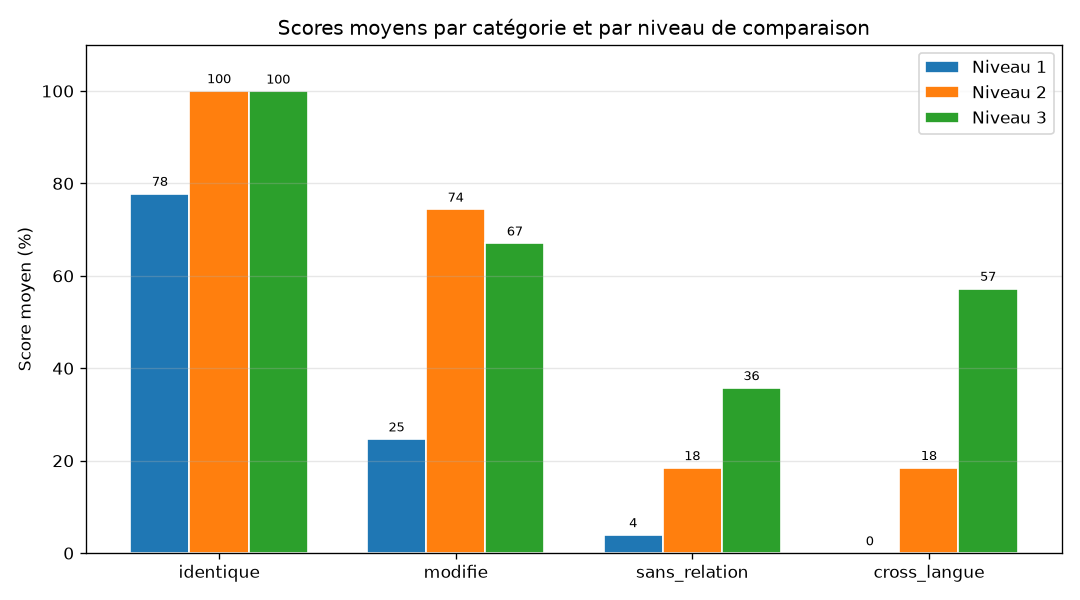
\includegraphics[width=0.62\linewidth]{figures/scores_moyens.png}
  \caption{Scores moyens par catégorie et par niveau (généré par
  \texttt{evaluation/plots.py}).}
\end{figure}

% ===========================================================================
\section{Limites de la solution}
% ===========================================================================

\begin{itemize}
  \item \textbf{Faux positifs du niveau 3 sur petits fichiers} : des
        programmes courts de même langage partagent des proportions
        structurelles proches (vecteurs dominés par \texttt{IF}/\texttt{LOOP}) ;
        la variation totale atténue le phénomène sans l'éliminer
        (précision $58{,}3\,\%$). D'où la recommandation des niveaux 1--2 pour
        un même langage, appliquée automatiquement en mode \emph{auto}.
  \item \textbf{Motifs algorithmiques heuristiques} : limités à une liste
        fermée et sensibles au style d'écriture ; une généralisation par
        apprentissage supervisé nécessiterait un corpus annoté.
  \item \textbf{Édition d'arbre simplifiée} : l'appariement glouton par
        catégorie n'est pas optimal (Zhang--Shasha exact reste coûteux) ;
        acceptable aux tailles observées grâce à la borne de profondeur.
  \item \textbf{Bibliothèques standard figées} : les listes blanches sont
        statiques ; une extraction dynamique des imports améliorerait la
        normalisation.
  \item \textbf{Scalabilité} : Winnowing et GST sont quasi linéaires, mais le
        coût de \emph{tree-sitter} croît avec la taille ; le mode répertoire
        compare chaque candidat indépendamment, sans matrice complète
        optimisée.
  \item \textbf{Validation} : l'évaluation repose sur un jeu étiqueté de 24
        scénarios, suffisant pour comparer les niveaux mais de taille modeste ;
        l'absence de tests unitaires automatisés rend les régressions
        silencieuses plus probables.
  \item \textbf{Dimension éthique} : un score de similarité n'est pas une
        preuve de plagiat ; il constitue une aide à la décision devant faire
        l'objet d'un examen humain critique.
\end{itemize}

\end{document}
